\section{Experiments}
\label{sec:experiments}

\subsection{Setup}
\label{sec:exp-setup}

\paragraph{Model.}
The DSA model used in our experiments was obtained through a two-stage training process starting from the base model of GLM-4.7-Flash\footnote{\url{https://huggingface.co/zai-org/GLM-4.7-Flash}}, a 30B-A3B MoE model with Multi-head Latent Attention~(MLA) and 47 layers. Its evaluation performance is comparable to that of the original GLM-4.7-Flash (see Table~6 in \citet{glm5}).

\paragraph{Training-free IndexCache.}
The greedy pattern search is guided by the per-token validation loss computed on SFT data with a batch size of 768 and a context length of 200K.

\paragraph{Training-aware IndexCache.}
A full DSA training pipeline starting from the base model requires substantial computational resources. Instead, we initialize directly from the GLM-4.7-Flash model and train it into a DSA model on SFT data with a context length of 200K. The training consists of a 1{,}000-step dense warm-up phase followed by a 4{,}000-step sparse training phase. This shorter pipeline closely matches the performance of full DSA training and suffices for evaluating IndexCache's training-aware component.

\paragraph{Evaluation.}
We include five long-context benchmarks: MRCR~v2~\citep{mrcr}, GraphWalks~\citep{graphwalks}, LongBench~v2~\citep{longbenchv2}, RULER~\citep{ruler}, and AA-LCR~\citep{aalcr}; four general \& reasoning benchmarks: AIME~2025~\citep{aime2025}, GPQA-Diamond~\citep{gpqa}, LiveCodeBench~v6~\citep{livecodebench}, and IFBench~\citep{ifbench}.
Evaluation setups are further detailed in Appendix~\ref{app:eval}.

\begin{table}[t]
\centering
\caption{%
    End-to-end inference performance of the 30B DSA model with IndexCache at two retention ratios.
    \textbf{Prefill time}: seconds (lower is better).
    \textbf{Decode per request}: tokens/s under single concurrency (higher is better).
    \textbf{Decode full}: total tokens/s (higher is better).
    Decode throughput is reported per GPU.
}
\label{tab:profiling}
\small
\begin{tabular}{lcccc}
\toprule
& 10K & 60K & 120K & 200K \\
\midrule
\multicolumn{5}{l}{\textit{Prefill time (s)} $\downarrow$} \\
\quad DSA & 0.57 & 3.38 & 8.57 & 19.5 \\
\quad + IndexCache (1/2) & 0.47 & 2.86 & 6.57 & 13.7 \\
\quad + IndexCache (1/4) & \textbf{0.45} & \textbf{2.59} & \textbf{5.66} & \textbf{10.7} \\
\midrule
\multicolumn{5}{l}{\textit{Decode throughput, per request (tok/s)} $\uparrow$} \\
\quad DSA & 73.5 & 67.0 & 63.0 & 58.0 \\
\quad + IndexCache (1/2) & 84.5 & 80.0 & 77.0 & 73.0 \\
\quad + IndexCache (1/4) & \textbf{91.0} & \textbf{89.5} & \textbf{88.0} & \textbf{86.0} \\
\midrule
\multicolumn{5}{l}{\textit{Decode throughput, full KV cache (tok/s)} $\uparrow$} \\
\quad DSA & 2700 & 613 & 341 & 197 \\
\quad + IndexCache (1/2) & 3070 & 750 & 431 & 253 \\
\quad + IndexCache (1/4) & \textbf{3310} & \textbf{840} & \textbf{498} & \textbf{297} \\
\bottomrule
\end{tabular}
\end{table}

\begin{figure}[t]
\centering
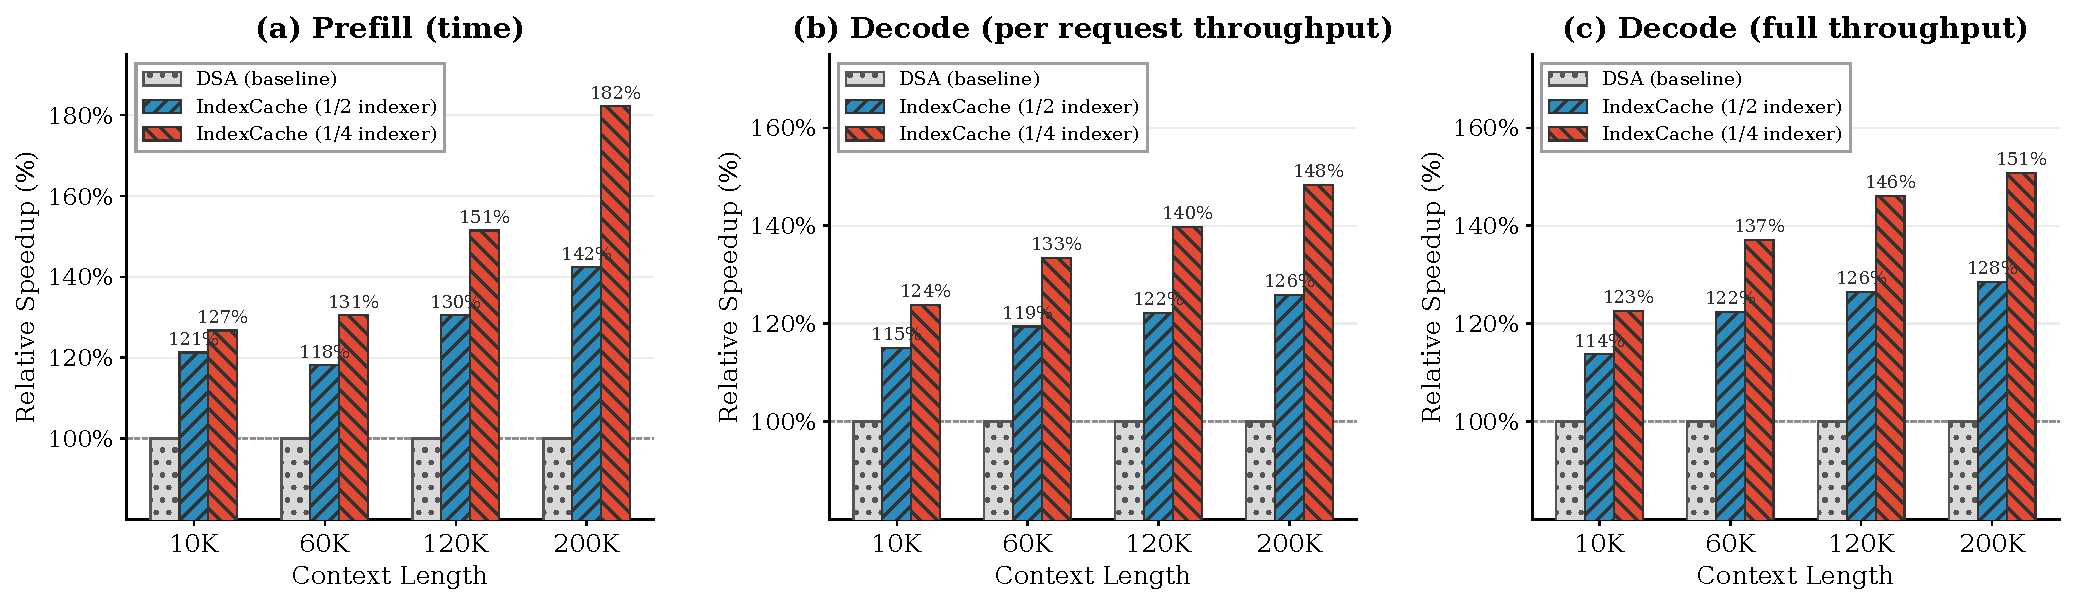
\includegraphics[width=\textwidth]{figures/profiling_speedup.pdf}
\caption{%
    Relative speedup of IndexCache over the DSA baseline across three inference settings on the 30B model.
    DSA baseline is normalized to 100\%.
}
\label{fig:profiling-speedup}
\end{figure}

\subsection{End-to-End Inference Speedup}
\label{sec:exp-profiling}
We measure end-to-end inference performance using the 30B-parameter DSA model served with \texttt{dp\_attention} enabled (\texttt{dp\_size=8}) in SGLang, running on an NVIDIA H100 node.
We compare the original DSA baseline against IndexCache at two retention ratios: 1/2 (half of the indexer layers retained) and 1/4 (a quarter retained).
We report three complementary metrics across context lengths of 10K, 60K, 120K, and 200K tokens:
(1)~\emph{prefill latency} which measures time-to-first-token;
(2)~\emph{per-request decode throughput} under single concurrency (single request on each GPU);
and (3)~\emph{total decode throughput} when the KV cache is fully utilized (${\sim}$800K tokens on each GPU).
Table~\ref{tab:profiling} and Figure~\ref{fig:profiling-speedup} summarize the results.

\paragraph{Prefill.}
IndexCache delivers substantial prefill acceleration that grows with context length.
At 200K tokens, IndexCache~(1/4) reduces prefill latency from 19.5s to 10.7s, achieving a \textbf{1.82$\times$} speedup, by eliminating 75\% of the indexer computations that dominate the prefill phase.
Even at 10K, where the indexer accounts for a smaller fraction of total compute, a 1.27$\times$ speedup is observed.
Extrapolating to longer contexts ($>$200K), IndexCache is expected to deliver even greater speedups.

\paragraph{Decode.}
The per-request decode throughput improvement is significant at long contexts.
At 200K, DSA's decode speed is 58 tok/s, while IndexCache~(1/4) achieves 86 tok/s, a \textbf{1.48$\times$} speedup.
This is because the decode phase in DSA involves a per-token indexer pass over the full context, which becomes the bottleneck at long sequences; IndexCache directly reduces this bottleneck.
When the KV cache is fully saturated, IndexCache~(1/4) improves total decode throughput by 22-51\% across context lengths, with the largest gains at longer contexts (197$\to$297 tok/s at 200K, a \textbf{1.51$\times$} increase).

We observe similar trends on the larger GLM-5 model (744B parameters), where IndexCache~(1/4) yields at least \textbf{1.3$\times$} improvement in both prefill latency and decode throughput at context lengths beyond 100K.
Overall, our end-to-end prefill latency and decode throughput suggest IndexCache is particularly valuable for the long-context scenario.


\subsection{Training-Free IndexCache Results}
\label{sec:exp-trainfree}

Table~\ref{tab:trainfree} reports results of training-free IndexCache on the same 30B DSA model, comparing three retention ratios: 1/2, 1/4, and 1/8, each under a uniform interleave baseline and a greedy-searched pattern (Appendix~\ref{app:pattern}).

\begin{table}[t]
\centering
\caption{%
Training-free IndexCache at 1/2, 1/4, and 1/8 indexer retention.
`Long' and `G\&R' aggregate benchmark scores.
We compare uniform interleaving against searched patterns.
}
\label{tab:trainfree}
% \small
\resizebox{\textwidth}{!}{%
\begin{tabular}{lcc ccccc ccccc}
\toprule
& \multicolumn{2}{c}{\textbf{Averages}} & \multicolumn{5}{c}{\textbf{Long-Context}} & \multicolumn{4}{c}{\textbf{General \& Reasoning}} \\
\cmidrule(lr){2-3} \cmidrule(lr){4-8} \cmidrule(lr){9-12}
\textbf{Config} & Long & G\&R & MRCR & GW & LB2 & RULER & LCR & AIME & GPQA & LCB & IFB \\
\midrule
Original DSA & 50.2 & 74.6 & 24.5 & \textbf{49.6} & 45.5 & \textbf{87.9} & 43.6 & 91.0 & 77.6 & \textbf{71.4} & 58.4 \\
\midrule
\rowcolor{mygray}1/2 Unif. IndexCache & 47.4 & 74.3 & 22.0 & 46.6 & 46.0 & 83.6 & 38.6 & 92.2 & 76.4 & 69.7 & \textbf{59.0} \\
\quad+Search pattern & \textbf{50.3} & 74.4 & \textbf{24.7} & 49.5 & \textbf{46.3} & 87.8 & 43.2 & 91.9 & 76.3 & 71.3 & 58.2 \\
\rowcolor{mygray}1/4 Unif. IndexCache & 43.0 & 73.8 & 17.7 & 37.2 & 43.1 & 79.2 & 37.8 & 91.3 & 75.7 & 69.4 & 58.9 \\
\quad+Search pattern & 49.9 & \textbf{74.9} & 25.1 & 47.4 & 45.7 & 87.6 & \textbf{43.8} & \textbf{92.6} & \textbf{78.6} & 70.0 & 58.3 \\
\rowcolor{mygray}1/8 Unif. IndexCache & 35.3 & 70.0 & 12.9 & 33.1 & 37.7 & 68.8 & 24.0 & 89.1 & 74.1 & 58.7 & 58.0 \\
\quad+Search pattern & 46.1 & 73.7 & 21.7 & 43.8 & 42.3 & 82.0 & 40.8 & 90.7 & 76.5 & 69.6 & 58.1 \\
\bottomrule
\end{tabular}%
}
\end{table}

\paragraph{Searched patterns close the gap on long-context tasks.}
Uniform interleaving at aggressive retention ratios incurs significant long-context degradation: 1/2 and 1/4 uniform interleaving drops Long~Avg by 2.8 and 7.2 points (50.2$\to$47.4 and 50.2$\to$43.0)
The greedy-searched pattern largely eliminates this deficit, recovering Long~Avg to 49.9 at 1/4 retention and to 50.3 at 1/2 retention, both comparable to the original DSA.
This confirms that \emph{which} indexer layers are retained matters far more than how many.
Nevertheless, when retaining only 1/8 of the indexer layers, we observe a substantial degradation: Long~Avg drops to 35.3 with uniform interleaving and to 46.1 with the searched pattern. While search-based IndexCache still markedly mitigates the loss caused by removing indexers, the resulting decline in long-context performance at this extreme sparsity becomes non-negligible.


\paragraph{Long chain-of-thought reasoning capabilities are preserved.}
Across all configurations except for uniform interleave at 1/8 ratio, G\&R~Avg stays within 1 point of the 74.6 baseline (73.7-74.9 vs.\ 74.6).
Notably, the 1/4 searched pattern \emph{improves} over DSA on AIME~2025 (92.6 vs.\ 91.0) and GPQA-Diamond (78.6 vs.\ 77.6), suggesting that removing redundant indexer computation may act as a mild regularizer during inference.
This confirms that IndexCache does not trade general reasoning ability for long-context efficiency.

\subsection{Training-Aware IndexCache Results}
\label{sec:exp-trainaware}

We perform training-aware IndexCache using the multi-layer distillation loss~(Section~\ref{sec:method-trainaware}) at two retention ratios: 1/2 and 1/4, both with uniform interleaving.
We further ablate two design choices at the 1/2 retention ratio: (1) replacing the uniform interleaving pattern with the greedy-searched pattern from Section~\ref{sec:exp-trainfree}, and (2) removing the cross-layer distillation loss (i.e., training each indexer only against its own layer's attention distribution).
Table~\ref{tab:trainaware} reports the evaluation results.
Note that the DSA baseline in this section is also trained using our shortened DSA training pipeline, which results in a small performance difference compared to the original DSA reported in Table~\ref{tab:trainfree}. 

\begin{table}[t]
\centering
\caption{%
    Training-aware IndexCache at 1/2 and 1/4 indexer retention with uniform interleaving.
    \emph{w/ searched pattern}: the greedy-searched pattern replaces uniform interleaving.
    \emph{w/o cross-layer loss}: each indexer is distilled only against its own layer.
}
\label{tab:trainaware}
\resizebox{\textwidth}{!}{%
\begin{tabular}{lcc ccccc cccc}
\toprule
& \multicolumn{2}{c}{\textbf{Averages}} & \multicolumn{5}{c}{\textbf{Long-Context}} & \multicolumn{4}{c}{\textbf{General \& Reasoning}} \\
\cmidrule(lr){2-3} \cmidrule(lr){4-8} \cmidrule(lr){9-12}
\textbf{Config} & Long & G\&R & MRCR & GW & LB2 & RULER & LCR & AIME & GPQA & LCB & IFB \\
\midrule
Original DSA & 51.0 & 74.2 & \textbf{24.7} & 49.1 & 46.9 & 87.3 & 47.0 & 88.8 & \textbf{79.4} & 70.5 & 57.9 \\
\midrule
1/2 Unif. IndexCache & \textbf{51.6} & \textbf{74.5} & 23.8 & \textbf{50.2} & \textbf{47.2} & 87.0 & \textbf{49.8} & 89.3 & 76.7 & \textbf{72.2} & \textbf{59.9} \\
\rowcolor{mygray}\quad w/ searched pattern & 50.6 & 73.6 & 23.9 & 48.1 & 47.1 & \textbf{87.5} & 46.6 & \textbf{89.6} & 78.6 & 68.5 & 57.7 \\
\rowcolor{mygray}\quad w/o cross-layer loss & 49.8 & 74.5 & 24.6 & 48.3 & 45.0 & 87.1 & 44.0 & 88.8 & 79.4 & 71.7 & 58.0 \\
1/4 Unif. IndexCache & 50.6 & 74.1 & 23.7 & 48.1 & 46.9 & 86.1 & 48.4 & 89.3 & 78.0 & 70.5 & 58.7 \\
\bottomrule
\end{tabular}%
}
\end{table}

\paragraph{Training-aware IndexCache matches DSA baseline.}
Uniform IndexCache with 1/2 ratio achieves a Long~Avg of 51.6, \emph{surpassing} the baseline (51.0), while G\&R~Avg remains comparable (74.5 vs.\ 74.2).
At 1/4 retention, both Long~Avg and G\&R~Avg are within 0.4\% of the baseline.
These results confirm that DSA can be trained to adapt to the sharing pattern.

\paragraph{The pattern sensitivity observed in training-free IndexCache vanishes with training.}
A striking contrast with Section~\ref{sec:exp-trainfree} emerges: uniform interleaving at 1/2 retention performs on par with and even slightly above the greedy-searched pattern (Long~Avg 51.6 vs.\ 50.6; G\&R~Avg 74.5 vs.\ 73.6).
Recall that in the training-free setting, the searched pattern was essential for recovering quality at aggressive retention ratios.
This is because, without retraining, certain layers are strongly coupled to their own indexer's top-$k$ selection; inheriting indices from an earlier layer introduces a distributional shift that causes sharp performance drops.
The greedy search in the training-free setting works precisely by avoiding these sensitive layers.
However, when the model is retrained with a sharing-aware objective, the \texttt{S}~layers learn to adapt their attention to inherited indices, and the retained indexers simultaneously learn to produce selections that generalize across their served layers.
This joint adaptation eliminates the layer-specific sensitivity entirely, allowing even a simple uniform pattern to match the full-indexer baseline.

\paragraph{Cross-layer distillation provides a meaningful benefit.}
Removing the cross-layer loss drops Long~Avg from 51.6 to 49.8, with AA-LCR falling from 49.8 to 44.0.
This confirms that the multi-layer distillation objective is practically beneficial: by training each indexer toward the centroid of its served layers' attention distributions, it learns a consensus top-$k$ that generalizes across layers rather than overfitting to a single one.

\subsection{Scaling Experiment}
\label{sec:scales}

\begin{table}[t]
\centering
\caption{%
    Preliminary results on GLM-5 (744B) with training-free IndexCache.
}
\label{tab:scaling}
\resizebox{0.95\textwidth}{!}{%
\begin{tabular}{lc ccccc}
\toprule
& \textbf{Long Avg} & \textbf{MRCR v2} & \textbf{GraphWalks} & \textbf{LongBench v2} & \textbf{RULER} & \textbf{AA-LCR} \\
\midrule
Original DSA & 78.4 & 71.1 & \textbf{92.7} & 64.5 & \textbf{97.7} & 66.2 \\
\midrule
\rowcolor{mygray}1/2 Unif. IndexCache & 78.1 & \textbf{72.8} & 90.2 & 65.1 & 97.6 & 64.6 \\
\quad+Searched pattern & \textbf{78.7} & 72.3 & 90.8 & \textbf{66.0} & 97.3 & 67.2 \\
\rowcolor{mygray}1/4 Unif. IndexCache & 72.7 & 65.8 & 74.9 & 62.2 & 96.2 & 64.6 \\
\quad+Searched pattern & 78.0 & 70.8 & 90.3 & 63.7 & 97.6 & \textbf{67.6} \\
\bottomrule
\end{tabular}%
}
\end{table}

We apply training-free IndexCache to GLM-5, a 744B-parameter (40B active) model that uses DSA by default. Table~\ref{tab:scaling} reports results on five long-context benchmarks.
The overall trends mirror the 30B findings: uniform interleaving degrades at aggressive retention, while the searched pattern recovers quality.
Interestingly, uniform interleaving at 1/2 retention happens to preserve Long~Avg (78.1 vs.\ 78.4), but this is likely coincidental, where the fixed alternating pattern simply avoids skipping the most critical indexer layers by chance.
The searched pattern provides consistently stable results: at 1/2 retention it slightly \emph{exceeds} the baseline (78.7 vs.\ 78.4), and at 1/4 retention it remains within 0.4 points (78.0 vs.\ 78.4).
We also conducted an all-round evaluation of IndexCache with 1/2 indexer retention across all tests on the Artificial Analysis Index, and its performance is nearly identical to that of the original GLM‑5 model (Figure~\ref{fig:glm5}).

We plan to apply training-aware IndexCache to this production-scale model in the near future. Given that the training-free variant already matches baseline quality, we are optimistic that training-aware adaptation will further solidify these gains and translate into concrete deployment-time efficiency benefits.
